\chapter{Introdução}

% [NOTA: Remover parágrafo redundante - esta informação já aparece nos objetivos]
A gestão medicamentosa em ambiente hospitalar constitui um dos processos mais críticos e complexos das instituições de saúde modernas. O Hospital da Misericórdia de Vila Verde (SCMVV), à semelhança de outras unidades hospitalares nacionais, enfrenta desafios significativos na coordenação entre prescrição médica, validação farmacêutica e administração por enfermagem. Este trabalho apresenta o desenvolvimento e implementação de um sistema integrado de gestão medicamentosa que visa resolver estas lacunas através de tecnologias modernas.

\section{Contexto e Enquadramento}

A gestão medicamentosa em ambiente hospitalar constitui um dos processos mais críticos e complexos do sistema de saúde \cite{kohn2000,berwick2008}. No Hospital da Santa Casa da Misericórdia de Vila Verde (SCMVV), a necessidade de modernização dos sistemas informáticos tornou-se evidente face aos desafios crescentes de segurança, eficiência e rastreabilidade.

\begin{figure}[htbp]
    \centering
    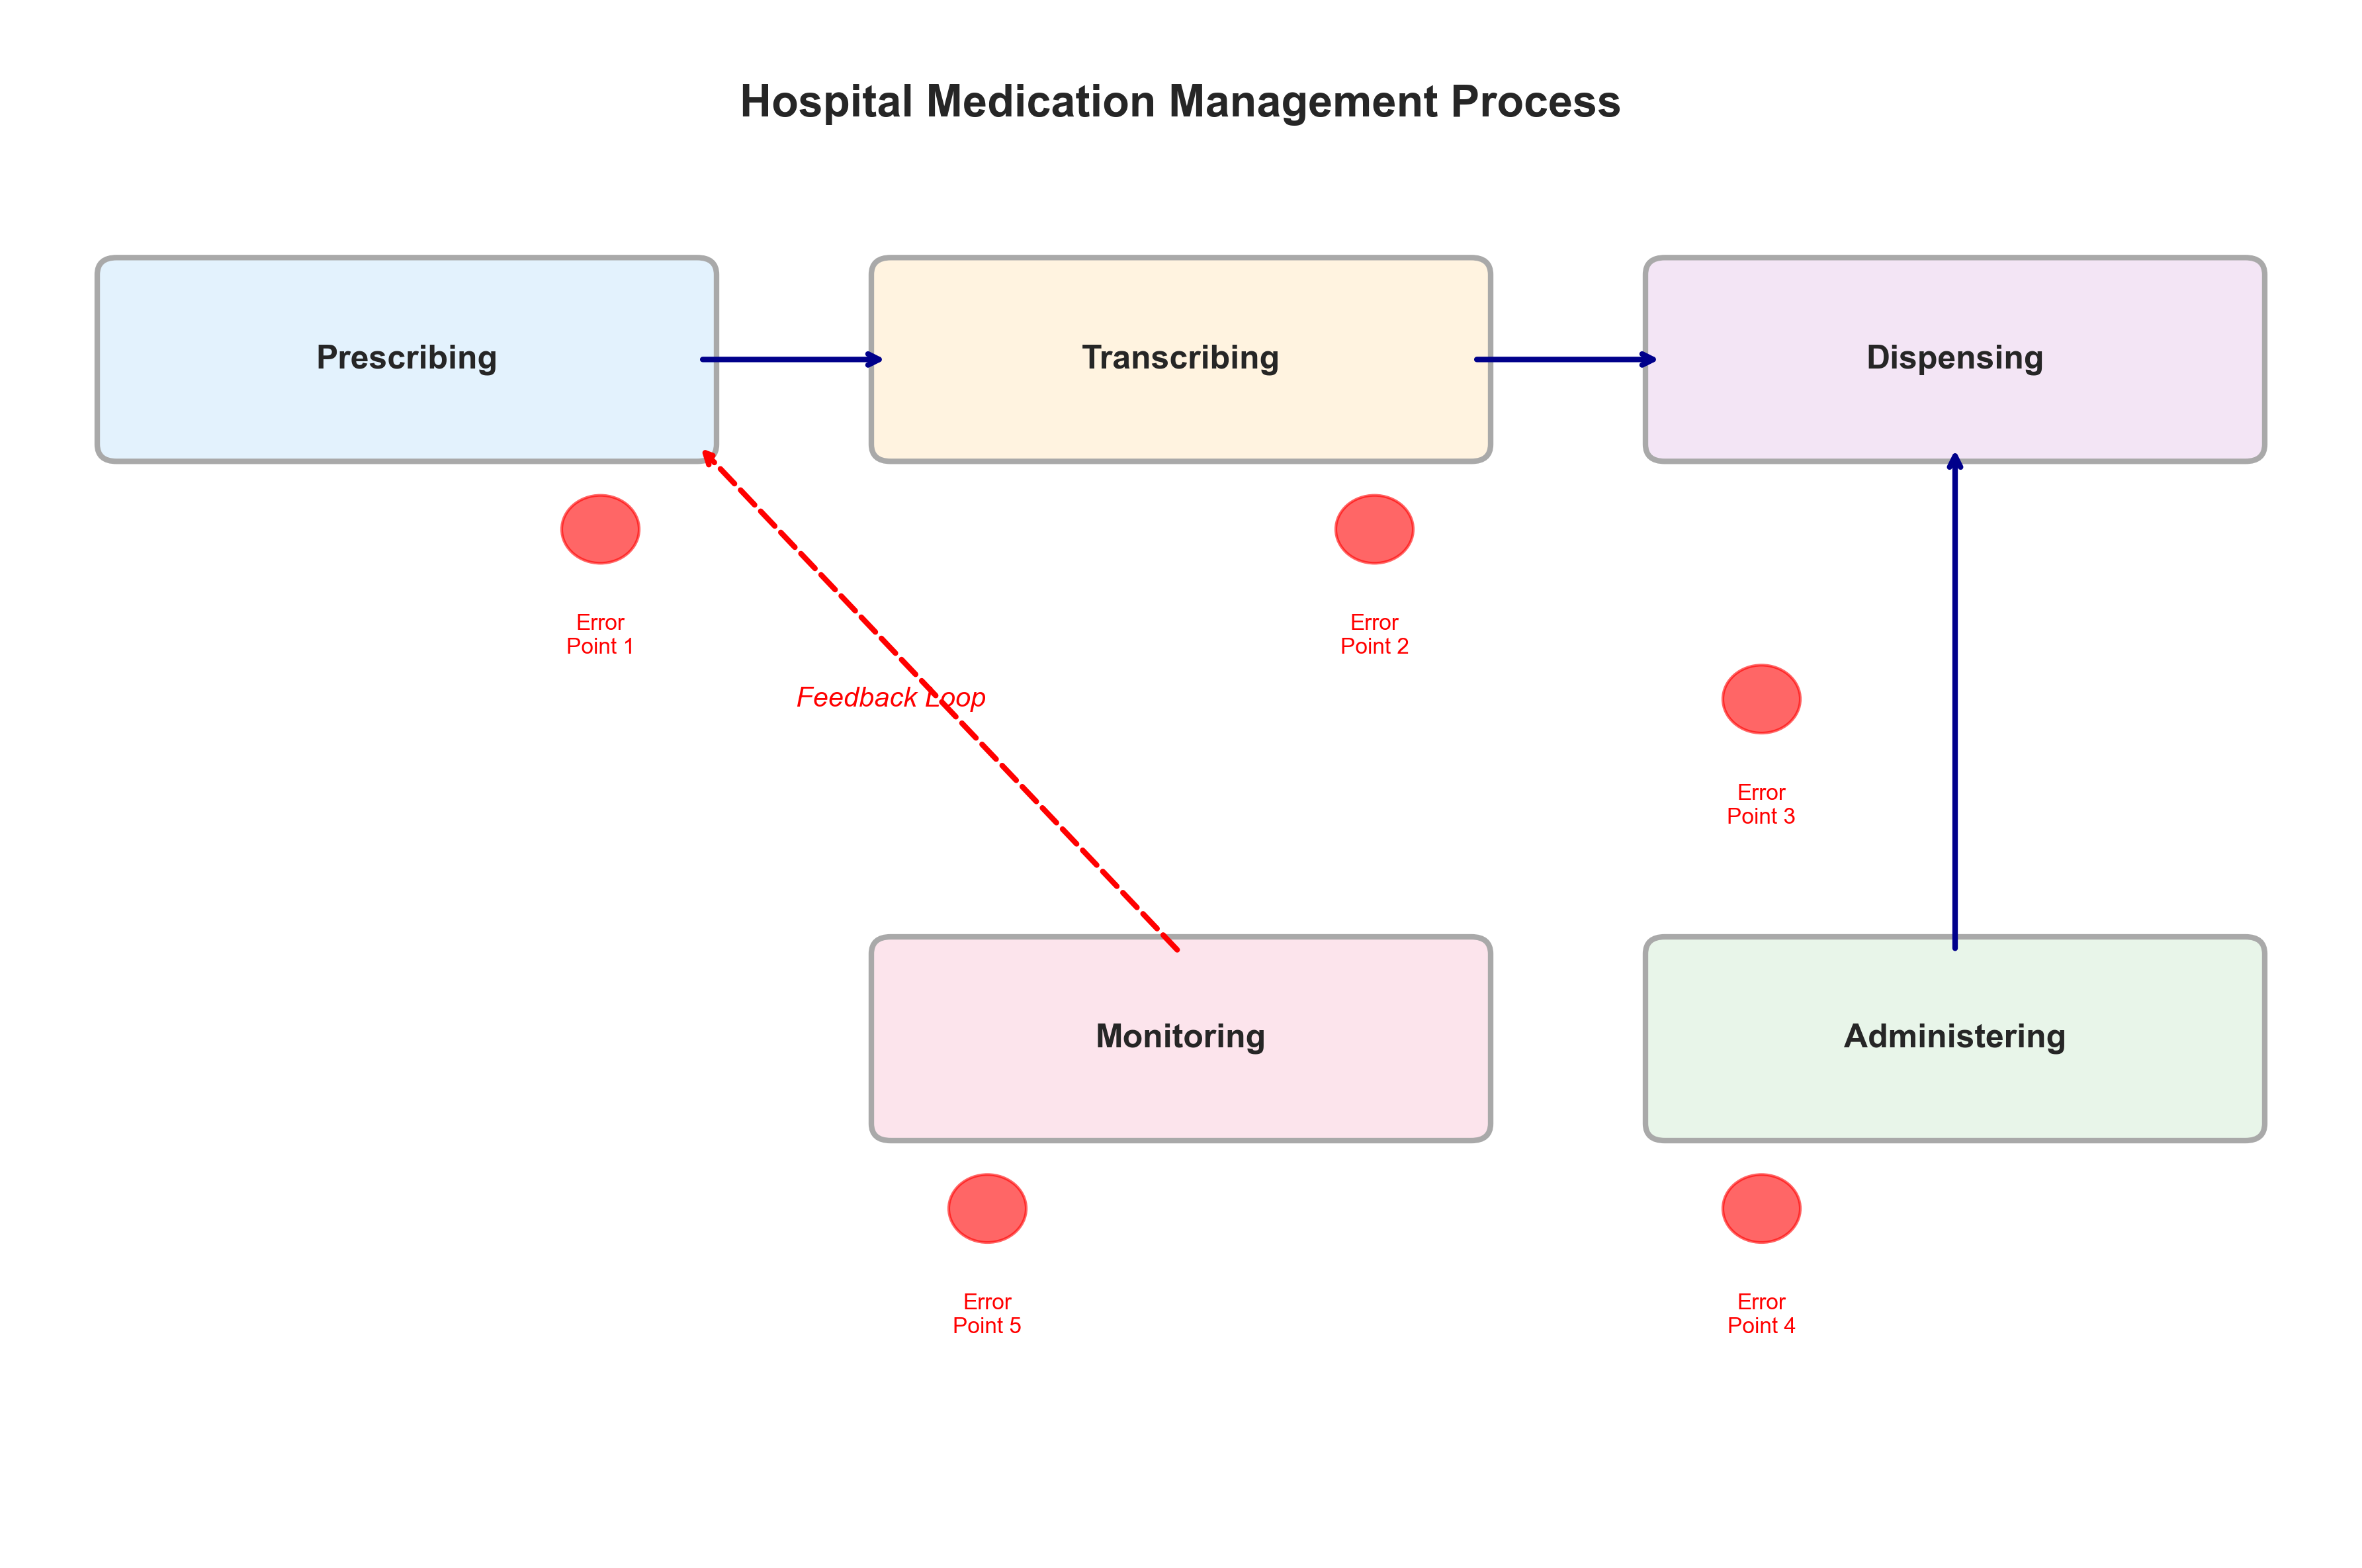
\includegraphics[width=0.9\textwidth]{images/generated/medication_flow_process.png}
    \caption{Hospital medication management process showing the five main stages and potential error points. Adapted from the medication use process framework \citep{austin2018,zheng2021}.}
    \label{fig:medication_flow}
\end{figure}

Os sistemas hospitalares portugueses operam frequentemente com soluções fragmentadas, desenvolvidas em diferentes épocas \cite{kazemi2016} e com tecnologias díspares. Na SCMVV, o sistema legado AIDA-PCE, implementado antes de 2010, continua operacional mas apresenta limitações significativas:

O sistema apresenta uma interface desatualizada que dificulta a navegação e aumenta significativamente o tempo necessário para prescrição médica. A ausência de validações automáticas em tempo real \cite{moss2015} compromete a segurança do paciente, enquanto a falta de integração com sistemas modernos de gestão hospitalar resulta em silos de informação e processos fragmentados. 

Adicionalmente, as dificuldades na geração de relatórios e análise de dados \cite{bowles2020} limitam a capacidade de monitorização e melhoria contínua. Os problemas de escalabilidade com o aumento do volume de pacientes evidenciam a necessidade urgente de modernização tecnológica.

% [INSERIR: Tabela 1.1 - Estatísticas de erros de medicação em hospitais portugueses (fonte: DGS)]

\section{Motivação e Relevância}

Segundo dados da Organização Mundial de Saúde \cite{who2017,who2022}, os erros de medicação afetam 1 em cada 10 pacientes \cite{who2017} hospitalizados globalmente. Em Portugal, embora não existam estatísticas oficiais consolidadas, estima-se que o impacto seja similar \cite{dgs2020}. A implementação de sistemas integrados de gestão medicamentosa \cite{shermock2023,vaghasiya2023} pode reduzir estes erros em até 85\% \cite{mahoney2007}.

% [DESENVOLVER: Adicionar dados específicos da SCMVV - número de camas, prescrições/dia, etc.]

\section{Objetivos}

\subsection{Objetivo Geral}
Desenvolver um sistema integrado de gestão medicamentosa que otimize os processos de prescrição, validação, dispensa e administração de medicamentos na SCMVV, garantindo maior segurança do paciente \cite{ciapponi2021} e eficiência operacional.

\subsection{Objetivos Específicos}

Para alcançar o objetivo geral, foram definidos cinco objetivos específicos fundamentais. Primeiro, modernizar a interface do sistema através do desenvolvimento de uma interface intuitiva e responsiva utilizando React \cite{misra2023} e Material-UI, com o objetivo de reduzir o tempo médio de prescrição. Segundo, implementar um sistema robusto de validação em tempo real para interações medicamentosas \cite{moss2015,belle2013} e dosagens, aumentando a segurança do paciente.

Terceiro, garantir rastreabilidade completa através do estabelecimento de auditoria abrangente de todas as operações \cite{european2016}, permitindo monitorização e análise retrospetiva. Quarto, integrar o sistema com SONHO, farmácia e outros sistemas hospitalares através de APIs RESTful \cite{mandl2020}, eliminando silos de informação. Finalmente, otimizar a performance do sistema através de técnicas avançadas de caching e otimização de queries Oracle \cite{jiang2014}.

\section{Contribuições do Trabalho}

Este trabalho apresenta contribuições significativas para o campo da gestão medicamentosa hospitalar. A principal contribuição técnica consiste numa arquitetura modular baseada em microserviços \cite{newman2021} que permite evolução independente de componentes, facilitando manutenção e extensibilidade futura. 

O desenvolvimento de um sistema de validação inteligente representa uma contribuição importante, implementando um motor de regras extensível para validação de prescrições \cite{amland2019} que pode ser adaptado a diferentes contextos hospitalares. A consolidação de múltiplos sistemas numa interface unificada \cite{bowles2020} constitui uma contribuição prática que melhora significativamente a experiência do utilizador.

Do ponto de vista técnico, o modelo de dados otimizado proporciona uma estrutura eficiente para consultas complexas em Oracle \cite{lin2018}, enquanto o framework de testes desenvolvido garante qualidade e confiabilidade através de uma suite completa de validações \cite{martin2017}.

% [INSERIR: Figura 1.2 - Arquitetura geral da solução proposta]

\section{Estrutura da Dissertação}

% [NOTA: Simplificar - remover descrições óbvias]
Os capítulos seguintes desenvolvem o trabalho realizado:
\textbf{Capítulo 2} apresenta o estado da arte;
\textbf{Capítulo 3} detalha o plano de trabalho;
\textbf{Capítulo 4} descreve a metodologia;
\textbf{Capítulo 5} apresenta os resultados;
\textbf{Capítulo 6} discute as implicações;
\textbf{Capítulo 7} conclui com trabalho futuro. 